\chapter{Graver bases} \label{2.Graver_bases}
\lhead{\emph{Graver bases}}  

% Chapter introduction
In this chapter we first define formally the Graver basis of a matrix, presenting and proving its main properties. After this, we present two algorithms for the general IP based on these properties, studying their complexity and main limitations. 

% Previous definitions
Before introducing the concept of Graver basis of a matrix, we define the partial order $\sqsubseteq$ in $\mathbb{R}^n$ by $u \sqsubseteq v$ if $u_i \cdot v_i \geq 0$ and $|u_i| \leq |v_i|$ for all i. Note that the condition $u_i \cdot v_i \geq 0$ means that $\sqsubseteq$ can only compare \textit{sign compatible} vectors, i.e., vectors with the same sign componentwise. We also introduce the notation $\mathcal{L}(A)$ for the integral kernel of a matrix excluding zero, i.e., $\mathcal{L}(A) := \{z \in \mathbb{Z}^n: Az = 0, z\neq0\}$.

% GRAVER BASIS OF A MATRIX
\begin{definition}[\textbf{Graver basis}]
The Graver basis $\mathcal{G}(A)$ of a given matrix $A \in \mathbb{Z}^{m \times n}$ is defined as the set of $\sqsubseteq$-minimal elements in $\mathcal{L}(A)$.
\end{definition}

\vspace{-5pt}
Graver bases were initially defined as \textit{universal integral test set} in \cite{GRAVER:1975} by Jack. E. Graver in 1975. They often appear defined in an equivalent way as the nonzero integral indecomposable elements in $ker(A)$. \emph{Indecomposable} in the sense that they can not be expressed as the sum of two sign compatible vectors. We now study their properties:

% Graver basis is a finite set
\begin{proposition}\label{GB_finite}
For every matrix A, $\mathcal{G}(A)$ is a finite set.
\end{proposition}
\vspace{-20pt}
\begin{proof}
Dickson's lemma states that every subset of $\mathbb{N}^n$ has a finite number of minimal elements with the order $\leq$ componentwise. It's easy to see that this implies that $\mathcal{L}(A)$ has a finite number of $\sqsubseteq$-minimal elements in every orthant. As the elements in different orthants are not comparable we have that $\mathcal{G}(A)$ is the union of $2^n$ finite sets, concluding the proof.
\end{proof}

% But they might grow exponentially
Unfortunately, the cardinality of $\mathcal{G}(A)$ may be exponential in $n$, the number of columns of $A$. This limits the explicit computation and usage of the Graver basis to only certain cases but doesn't limit its theoretical properties. The most important of these properties is expressed in the following proposition:

% Graver bases as universal integral test sets
\begin{proposition}\label{GB_test_set}
Every integral element in $ker(A)$ can be expressed as positive integral linear combination of sign compatible elements in $\mathcal{G}(A)$.
\end{proposition}
\vspace{-20pt}
\begin{proof}
The proof is by induction on the well partial order $\sqsubseteq$. For the base case we see that given $u \in \mathcal{L}(A)$ $\sqsubseteq$-minimal then $u$ belongs to $\mathcal{G}(A)$ and the result holds.

For the induction case lets take $u \in \mathcal{L}(A)$ not $\sqsubseteq$-minimal. Therefore there exists $u_1 \in \mathcal{L}(A)$ such that $u_1 \sqsubseteq u, u_1 \neq u$. We take $u_2 = u - u_1$. Note that thanks to the definition of $\sqsubseteq$ $u$, $u_1$ and $u_2$ are sign compatible and thanks to $u \neq u_1$ necessarily  $u_1,u_2 \sqsubset u$. With this appreciations, the proof concludes after applying the induction hypothesis:\\
\vspace{-30pt}
\begin{center}
    $u = u_1 + u_2 = \sum \alpha_{1i}g_{1i} + \sum \alpha_{2i}g_{2i} = \sum \alpha_{j}g_{j}$
\end{center}
\end{proof}

This proposition is the reason why Graver bases were introduced as \textit{universal integral test set}. It ensures that, given any feasible point, the whole feasible region can be expressed in terms of elements in $\mathcal{G}(A)$. Note that thanks to requiring positive coefficients and sign compatible elements we avoid cancellations in every component. 

In the next proposition we see how, thanks to this property, we can do an optimality test for any feasible point using only elements in the Graver basis.

% Graver bases optimality test
\begin{proposition}\label{GB_optimality_test}
Given a feasible point $z$ of the IP, $z$ is not optimum if and only if there exists $g \in \mathcal{G}(A)$ s.t. $c^tg > 0$ and $l \leq z + g \leq u$.
\end{proposition}
\vspace{-20pt}
\begin{proof}
If there exists $g \in \mathcal{G}(A)$ such that $c^tg > 0$ is clear that $z + g$ is a feasible point which strictly improves the objective function, so $z$ is not an optimum. 

For the other implication, if z is not an optimum we can take a feasible point $y$ improving $z$. Thanks to the previous proposition there exist $g_i \in \mathcal{G}(A)$, $\alpha_i \geq 0$ s. t. $(y - z) = \sum \alpha_i g_i$. Then $0 < c^t(y - z) = \sum \alpha_i c^t g_i$ so at least one $g_i \in \mathcal{G}(A)$ verifies $c^tg_i > 0$. Finally, $z + g_i$ is feasible because thanks to $\alpha_i \geq 0$ and $g_i$ being sign compatible with $y - z$ for all $i$ we have: $l \leq z \leq z + g_i \leq z + \sum \alpha_i g_i = y \leq u$.

\end{proof}

% GRAVER BASIS GREEDY AUGMENTATION ALGORITHM
\section{Graver basis greedy augmentation algorithm}

We now consider how to solve the general IP with the help of Graver bases. Note that proposition \ref{GB_optimality_test} doesn't only give us an optimality test but also provides us an improvement direction if the feasible point is not optimal. We can follow that improvement direction to get a better feasible point and then repeat this process. That is the idea of the following procedure (introduced in \cite{GRAVER:1975}):


\textbf{General IP algorithm using Graver basis} \label{GB_greedy_algorithm}
\vspace{-8pt}
\begin{enumerate}
    \item From a feasible solution $z_i$
    \item Find $g^*$ optimum for the augmentation step problem: \vspace{4pt}\\
          $max\{c^tg : g \in \mathcal{G}(A), l \leq z_i + g \leq u \}$ \vspace{4pt}
    \begin{itemize}
        \item $c^tg^* \leq 0 \implies z_i$ optimal solution.
        \item $c^tg^* > 0 \implies$ $g^*$ improvement direction, loop back to 1 with:\\ $z_{i+1} = z_i + \lambda \cdot g^*$ with the biggest $\lambda$ respecting the bounds.
    \end{itemize}
\end{enumerate}

% TODO: Reference for the suitable polynomail bounds result!
Note that the algorithm finishes in a finite number of steps thanks to the lower and upper bounds $l$ and $u$. We can assume the bounds are finite and, this way, the objective function is also bounded. Since every iteration we are strictly increasing the objective function, no infinite loop is possible. As stated in \cite{HEMMECKE:2011}, it is always possible to add suitable polynomial upper and lower bounds without excluding some optimal solution if any, so assuming $l$ and $u$ to be finite is no loss of generality.

% Algorithm complexity
The question that arises now is the complexity of this algorithm. It was analyzed in \cite[Theorem 3.3]{LHOW:2006} showing that it's polynomial. This of course doesn't mean we have a polynomial algorithm for the general IP, it means that, given an IP along with its Graver basis, we have a polynomial algorithm in this input size. The complexity of the problem remains in computing the Graver basis which, as we announced, may be exponential. This makes the algorithm non-viable but for small matrices. 

% TODO: If appendix A added, uncomment!
%In the Appendix A we go further to analyze how to compute the Graver basis of a given matrix and we introduce the tool \href{https://4ti2.github.io/}{4ti2}.

Another way to estimate the complexity of the algorithm is using \cite[Theorem 2.b]{HOW:2009}, which precises that the number of augmentation steps is polynomial. Assuming the Graver basis is given as part of the input, we could solve any augmentation step by iterating over the elements in $\mathcal{G}(A)$, checking the constraints and the objective function, which has complexity $n \cdot |\mathcal{G}(A)|$. Therefore, if the Graver basis is given the algorithm is polynomial in $n \cdot |\mathcal{G}(A)|$.


% GRAVER BASIS BOUND AUGMENTATION ALGORITHM
\section{Graver basis bound augmentation algorithm}

Up to this point we have seen how Graver bases allow a straightforward algorithm for the general IP. However, we have also seen that its main drawback is that it requires the explicit computation of the Graver basis. In this section we show how we can avoid computing the Graver basis thanks to bounds for the $\ell_1$-norm of its elements.

% Graver basis bounds
\label{GB_bounds}
\begin{proposition}[\textbf{Graver basis bounds}]
Given $A \in \mathbb{Z}^{mxn}$ and $\Delta$ an upper bound for the absolute value of each component of $A$, for every $g \in \mathcal{G}(A)$:
\vspace{-10pt}
\begin{itemize}
    \item $||g||_1 \leq m^{m/2}\Delta^m\cdot(n - m)$ \hspace{10pt}[Onn 2010]
    \item $||g||_1 \leq (2m \Delta + 1)^m$ \hspace{41pt}[Eisenbrand,Hunkenschröder,Klein 2018]
\end{itemize}
\end{proposition}

We refer to \cite{ONN:2010} and \cite{EISENBRAND:2018} for the proofs. Note that both bounds are exponential in the number of rows of $A$ but the second one has the advantage of being independent in the number of columns. This will be a key fact in the next chapter.

% Idea behind the augmentation algorithm
Why should bounds to the Graver bases help? Because thanks to the proposition \ref{GB_optimality_test}, the search of an improvement direction can be restricted to the elements in the Graver basis and, thanks to the bounds, we can restrict our search space without excluding any element of the Graver basis. This is the idea of the following algorithm \cite{HEMMECKE:2011}:

\vspace{10pt}
\begin{figure}[h]
\centering
\begin{minipage}[b]{0.45\textwidth}
    \centering
    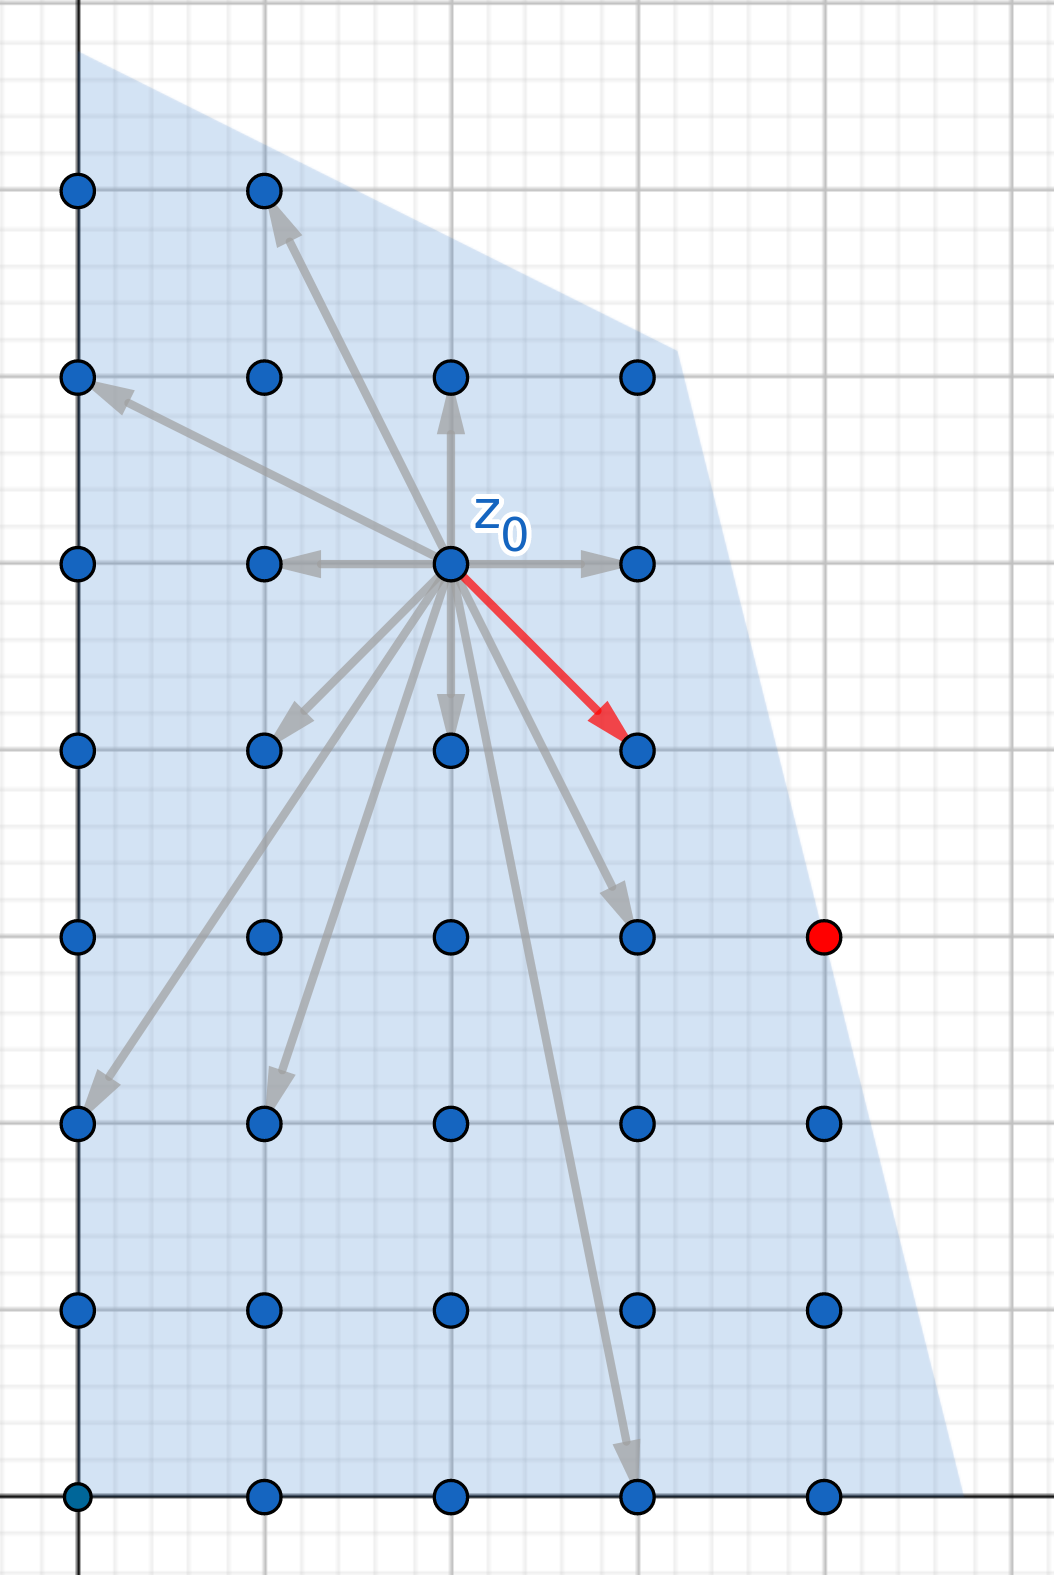
\includegraphics[width=0.9\textwidth]{images/IP(1).png}
    \caption{Feasible region}
\end{minipage}
\hfill
\begin{minipage}[b]{0.45\textwidth}
    \centering
    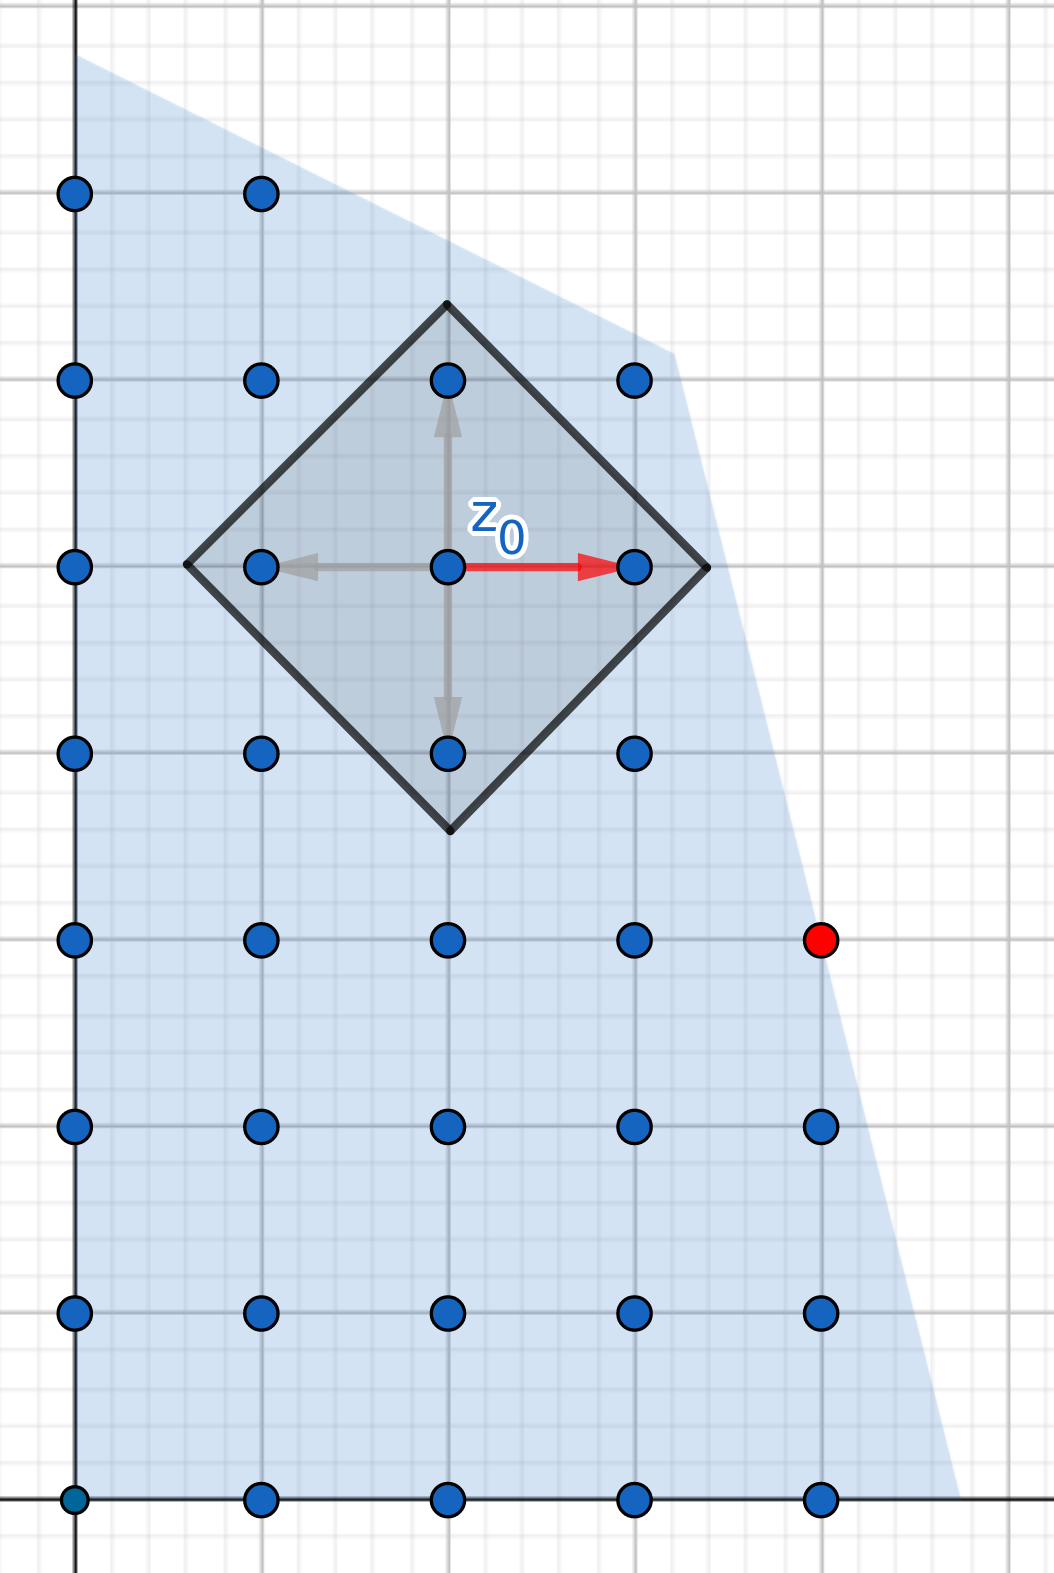
\includegraphics[width=0.9\textwidth]{images/IP.png}
    \caption{Bounded region}
\end{minipage}
\end{figure}

% Graver basis bound augmentation algorithm
\newpage
\label{GB_bound_algorithm}
\textbf{General IP algorithm using Graver basis norm bound}
\vspace{-8pt}
\begin{enumerate}
    \item From a feasible solution $z_i$
    \item Find $g^*$ optimum for the augmentation step problem: \vspace{4pt}\\
          $max\{c^tg : Ag = 0, l-z_i \leq g \leq u-z_i, g \in \mathbb{Z}^n, ||g||_1 \leq ||\mathcal{G}(A)|| \}$ \vspace{4pt}
    \begin{itemize}
        \item $g^* = 0 \implies z_i$ optimal solution.
        \item $g^* \neq 0 \implies$ $g^*$ improvement direction, loop back to 1 with:\\
        $z_{i+1} = z_i + \lambda \cdot g^*$ with the biggest $\lambda$ respecting the bounds.
    \end{itemize}
\end{enumerate}

% Algorithm complexity
As we advanced, the main advantage of this algorithm is that it doesn't require the explicit computation of the Graver basis. However, the complexity is totally dependent on the added restriction $||g||_1 \leq ||\mathcal{G}(A)||$ and, as we saw in the proposition \ref{GB_bounds}, the only bounds we have for the general case are exponential. This means that for the general IP the lower and upper bounds are much more restrictive than the Graver basis bound and therefore we have to explore the whole feasible region.

In certain cases we can get a much tighter bound for the Graver basis elements and this can help us to get a faster algorithm. The \emph{N-Fold IP} is an iconic example.